\section{Part B: Sinusoidal PWM}
\subsection{Q1}
%simulation from 90% speed to 100% speed. Plot speed vs time, 3 phase line to line voltages, 3 phase line currents, torque vs time, d-q currents, transition time

In the Fig \ref{fig:s1} below, we can observe the speed vs time graph of the pmsm motor. Here, we can see that the motor is speeding up from its 90\% rated speed to its rated speed. 

\begin{center}
\begin{figure}[H]
\centering
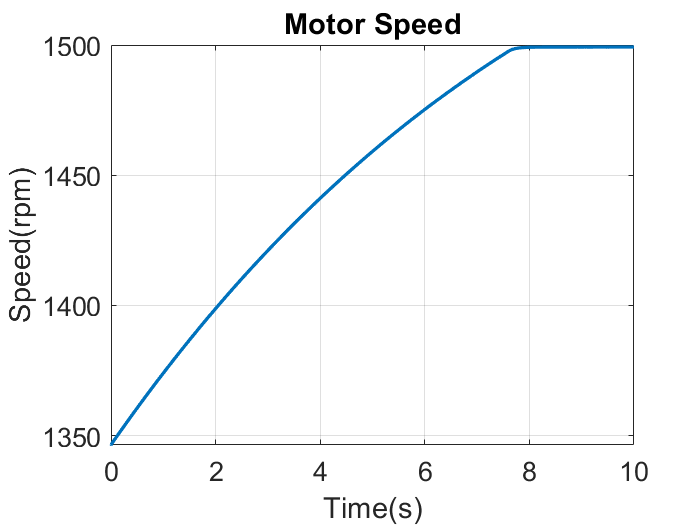
\includegraphics [width= 9 cm]{figs/Partb-1-hiz.png}
\caption{Speed vs time graph of the motor} 
\label{fig:s1} 
\end{figure}
\end{center}

In the Fig. \ref{fig:3line_V} and Fig. \ref{fig:3line_1V} below, we can observe the line to line voltage vs time. System does not reach the voltage limit since it is not on the maximum torque line. Nevertheless, it is very close to voltage limit.

\begin{figure}[H]
        \centering
        \begin{subfigure}[b]{0.475\textwidth}
            \centering
            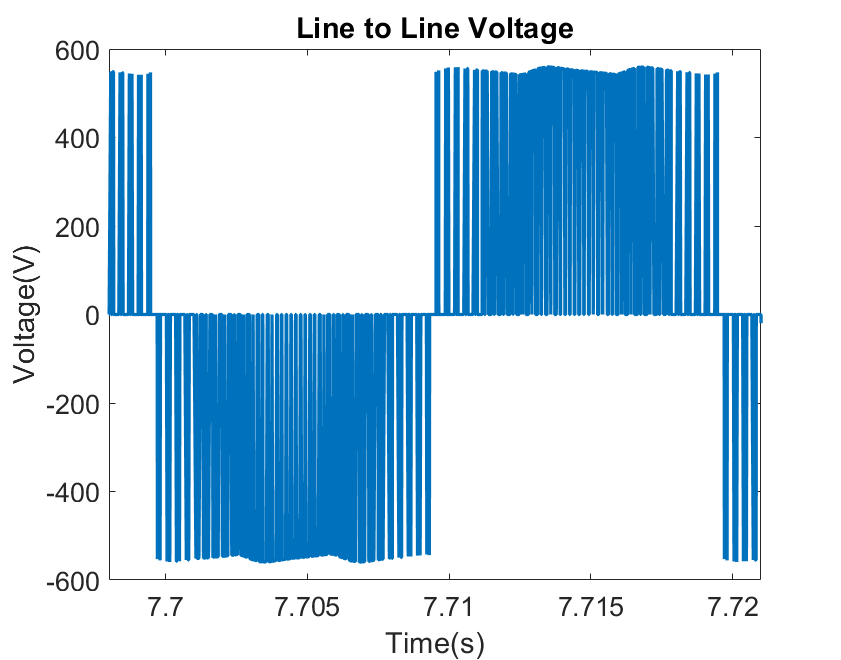
\includegraphics[width = 8 cm]{figs/ltol.png}
            \caption{Line to line voltage}
            \label{fig:3line_V}
        \end{subfigure}
        \hfill
        \begin{subfigure}[b]{0.475\textwidth}  
            \centering 
            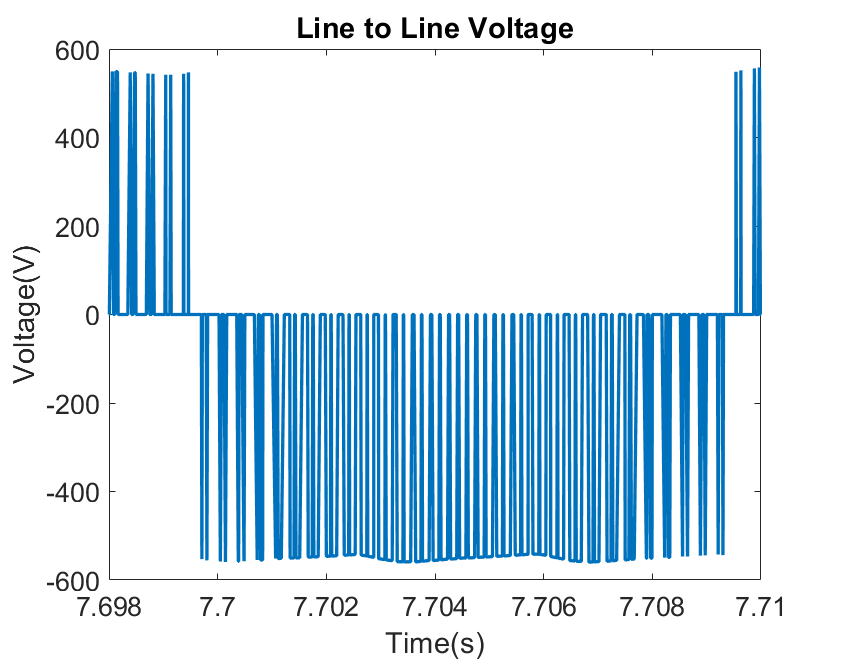
\includegraphics[width = 8 cm]{figs/partb-1-linetoline.png}
            \caption{Line to line voltage, one cycle}
            \label{fig:3line_1V}
        \end{subfigure}
        \caption{Line to line voltage general (a) and one cycle (b)}
        \label{fig:3phase}
        \end{figure}
        
In the Fig. \ref{fig:3phase_current} below, we can observe the phase currents vs time. At transient the currents decrease to their steady state value.

\begin{figure}[H]
        \centering
        \begin{subfigure}[b]{0.475\textwidth}
        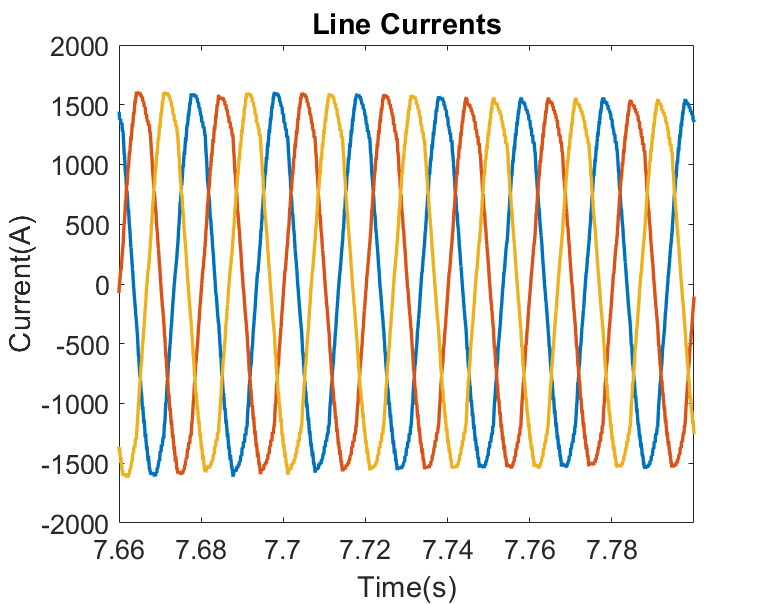
\includegraphics[width = 7 cm]{figs/Partb-1-phasecurrents.png}
        \caption{Line current, focused}
        \label{fig:3phase1}
        \label{fig:id}
        \end{subfigure}
        \hfill
        \begin{subfigure}[b]{0.475\textwidth}  
            \centering
        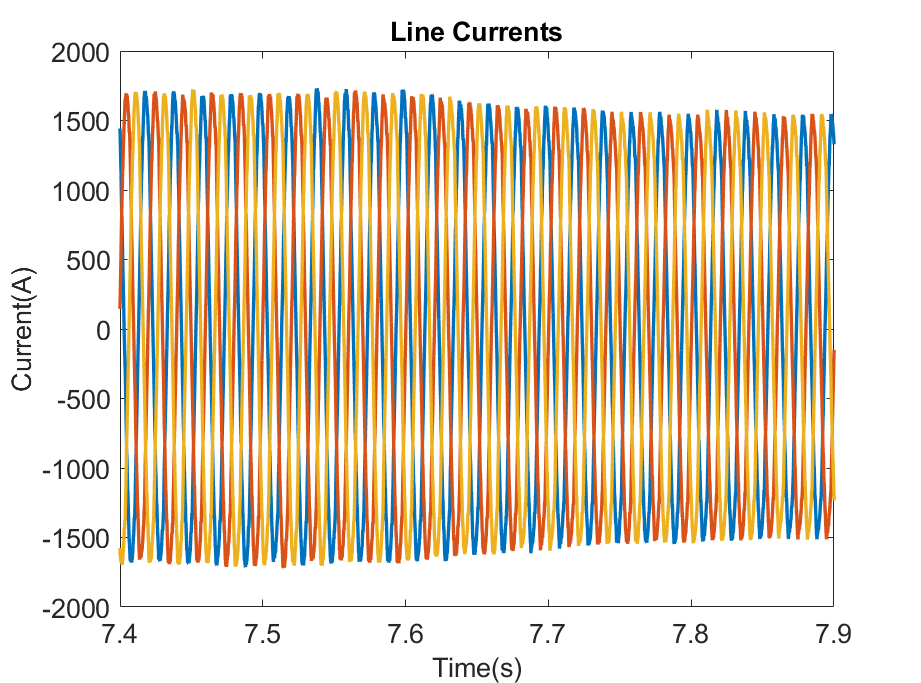
\includegraphics [width= 8cm]{figs/linecurrent_partb.png} 
        \caption{Line currents} % buraya alttaki gelecek oldu sanırım
        \label{fig:3phase2}
        \end{subfigure}
        \caption{Line current focused (a) and general (b)}
        \label{fig:3phase_current}
        \end{figure}
        
In the Fig. \ref{fig:t1} below, we can observe the machine torque vs time graph. It shows that the torque is increasing due to the load characteristic. In the Fig. \ref{fig:id} below, we can observe the $I_q$ and $I_d$ currents of the motor.


\begin{figure}[H]
        \centering
        \begin{subfigure}[b]{0.475\textwidth}
            \centering
        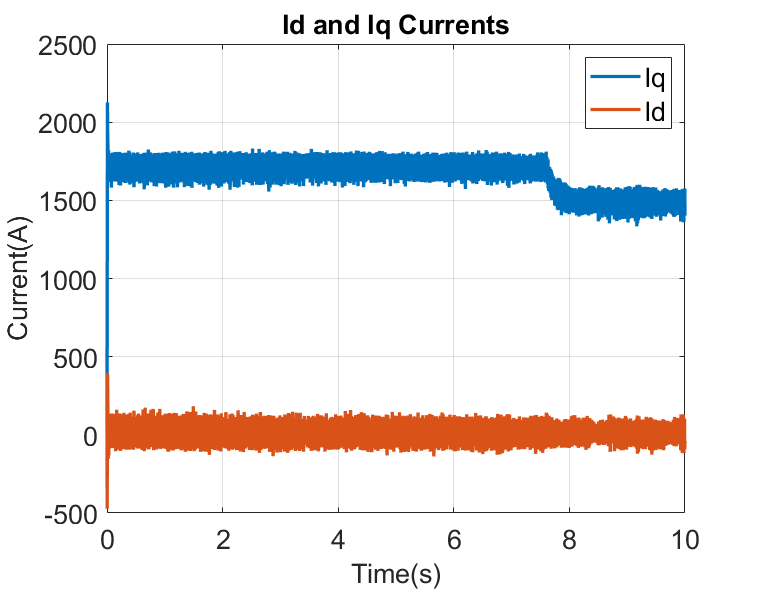
\includegraphics [width= 8 cm]{figs/Partb-1-IdIq.png}
        \caption{Motor currents in the d-q reference frame }
        \label{fig:id}
        \end{subfigure}
        \hfill
        \begin{subfigure}[b]{0.475\textwidth}  
            \centering
        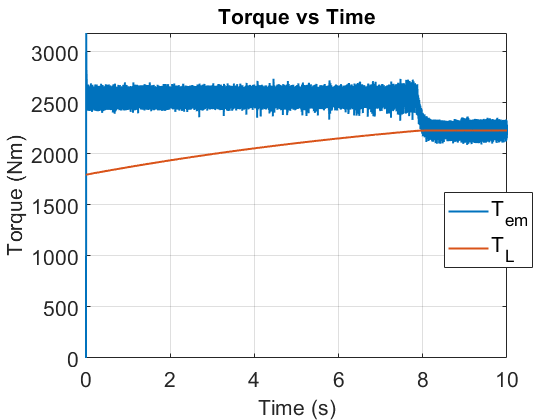
\includegraphics [width= 8cm]{figs/torque_new.png} % 
        \caption{Torque vs time graph of the motor}
        \label{fig:t1}
        \end{subfigure}
        \caption{d-q currents of the stator (a) and torque vs time (b)}
        \label{fig:3phase_torque}
        \end{figure}

We can see from the Fig. \ref{fig:3phase_torque}, the motor $i_q$ current and motor torque are directly proportional to each other. When we are in the transient, i.e. we are speeding the motor up, we apply maximum possible current which is $1700A$, when we reach the final speed, the apply steady state current which can supply enough current to operate the motor in constant speed. The noise is due to the controllers.

We can see that the time to go from 90\% to its rated speed is 7.5 seconds!

\subsection{Q2}
% when rated speed, make TL = 0, what happens, show graphs

In the Fig. \ref{fig:tl0_torque} below, we can observe the machine torque vs time graph. It shows that the torque is decreasing after time step $t=2s$ where we decrease the load torque to zero.

\begin{center}
\begin{figure}[H]
\centering
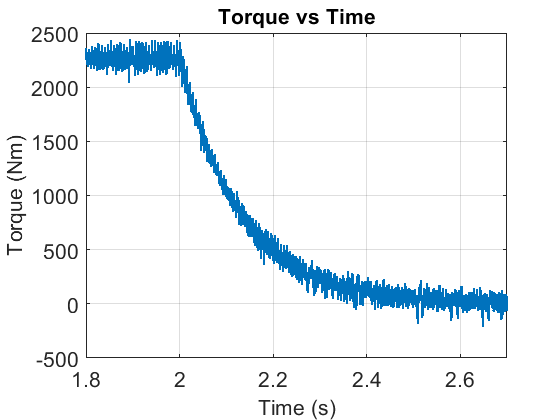
\includegraphics [width= 10 cm]{figs/TL0_torque.png}
\caption{Torque vs time graph of the motor}
\label{fig:tl0_torque}
\end{figure}
\end{center}

In this part, we lower the mechanical torque to the zero as we operating in rated conditions. we expect our phase currents to decrease and of course the $i_q$ current which deploys torque to decrease. 

In the Fig. \ref{fig:3phase_c} below, we can observe the phase currents vs time
        
        \begin{figure}[H]
        \centering
        \begin{subfigure}[b]{0.475\textwidth}
              \centering
        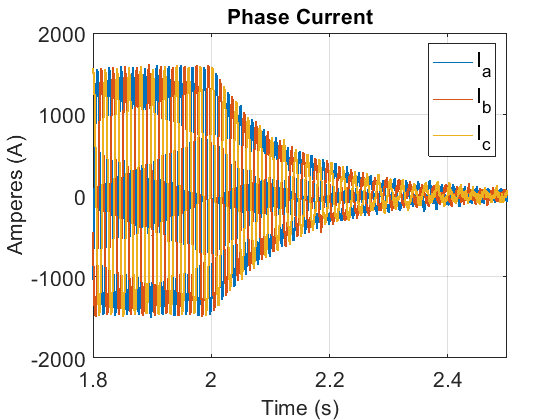
\includegraphics[width = 8 cm]{figs/TL0_phase.png}
        \caption{Motor line currents during transient}
        \label{fig:tl0_p}
        \end{subfigure}
        \hfill
        \begin{subfigure}[b]{0.475\textwidth}  
            \centering
        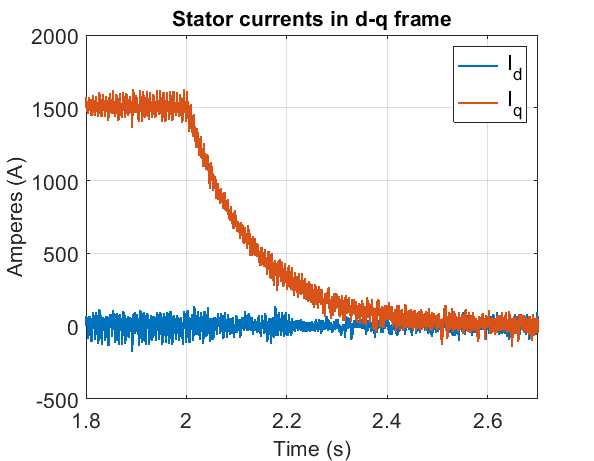
\includegraphics[width = 8 cm]{figs/TL0_dq.png}
        \caption{Motor stator d-q currents during transient}
        \label{fig:tl0_dq}
        \end{subfigure}
        \caption{Line to line voltage general (a) and one cycle (b)}
        \label{fig:3phase_c}
        \end{figure}
        
We can observe that the phase currents are lowering due to decrease in the torque. We know that the torque is directly proportional to the $i_q$ current, and a decrease in the $i_q$ while keeping $i_d$ constant will decrease line currents. After the transient, we have a noise in the line currents due to the inertia of the motor and the noise in the controllers.
        
As we observe, the $I_q$ current was it in rated value to apply rated torque at rated speed, then suddenly we decrease the load torque. Due to the controller, $i_q$ current decreases to $0$ where it provides zero torque, however, there are noise due to the controller circuit and motor itself.

\subsection{Q3}
%when no load, reverse the reference, if feasible? design a braking resistor, plot speed vs time,  3 phase line currents, d-q currents, dc link voltage,  

We know that during the braking time, the motor supplies current to the utility side, and if we do not have a full quadrant operation or back to back rectifiers, it is not possible to supply energy from load to the grid. In this case of operation as we have in this project, it is not possible to have a current into the grid because of the diode rectifier. So, the solution must be braking resistance. During transient time, the energy stored on the load and the motor can be discharged through this resistor. It prevents the circuit from burn-outs and excessive heating. The braking resistance selection of us is $R = 0.5 \ohm$. We can observe the braking resistance schematic below in the Fig. \ref{fig:brake}. As we follow, we sense the voltage on the capacitor, and when it exceeds 560V, we start to discharge the capacitor over the brake resistance. Here, we simulate the circuit to obtain maximum voltage of 600V during transient time. As we know, the larger resistance mean the greater peak voltage on the capacitor, so we should be careful when selecting the brake. As we mentioned above, the braking resistance is $R_{brake} = 0.5\ohm$

\begin{center}
\begin{figure}[H]
\centering
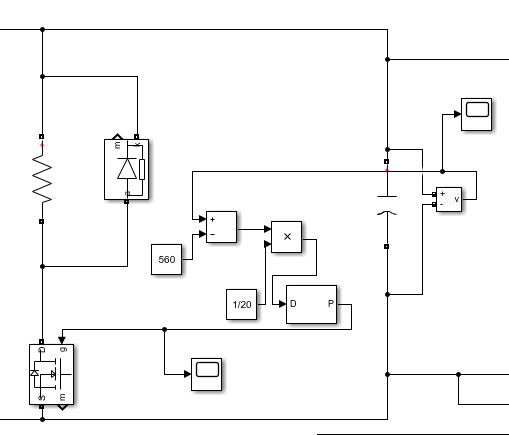
\includegraphics [width= 8 cm]{figs/brake.png}
\caption{Braking resistance circuitry}
\label{fig:brake}
\end{figure}
\end{center}

In the Fig. \ref{fig:rev1} we can observe that after we reverse the reference speed at time $t=1$ the motor speed decreases to 0, and then reversely increases to its final value. Meanwhile, due to the reversal, a negative torque is applied from the motor and it creates a current in the negative direction. This current should be discharged in order to prevent burnouts in the circuitry. Because of this simple phenomenon we introduce a braking resistance to the circuit.

\begin{figure}[H]
        \centering
        \begin{subfigure}[b]{0.475\textwidth}
            \centering
            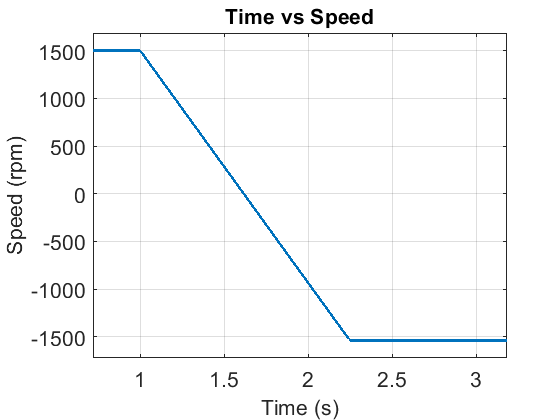
\includegraphics[width = 8 cm]{figs/reverse_speed.png}
            \caption{Speed }
            \label{fig:r_s}
        \end{subfigure}
        \hfill
        \begin{subfigure}[b]{0.475\textwidth}  
            \centering 
            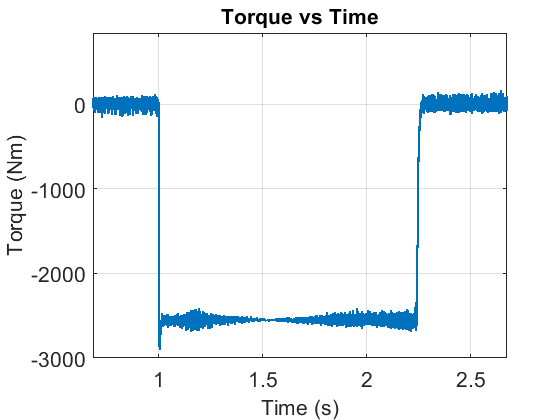
\includegraphics[width = 8 cm]{figs/reverse_torque.png}
            \caption{EM Torque}
            \label{fig:r_t}
        \end{subfigure}
        \caption{Reversal, speed vs time (a), electromechanical torque vs time (b)}
        \label{fig:rev1}
        \end{figure}

In the Fig. \ref{fig:rev_line1} below, we can easily observe that at the steady state we have only noise in the line currents, then when we reverse the speed reference, current is produced in the motor in order to reverse the motor. It deploys power to the utility side as we discussed before. In the Fig. \ref{fig:r22} we can see that the frequency of the current decreases to the zero and then increases again. This is due to the reducing speed of the motor and speeding up again.       
        
        
\begin{figure}[H]
        \centering
        \begin{subfigure}[b]{0.475\textwidth}
            \centering
            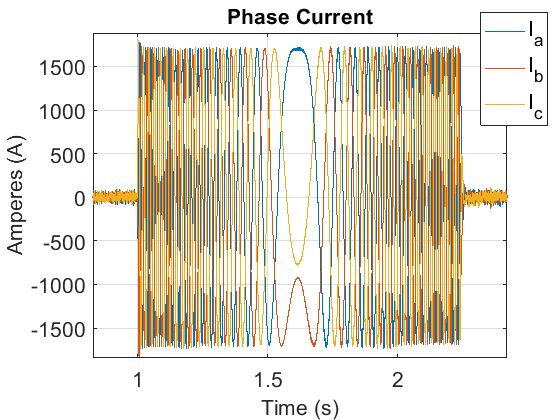
\includegraphics[width = 8 cm]{figs/reverse_phase2.png}
            \caption{Line currents during reversal}
            \label{fig:r11}
        \end{subfigure}
        \hfill
        \begin{subfigure}[b]{0.475\textwidth}  
            \centering 
            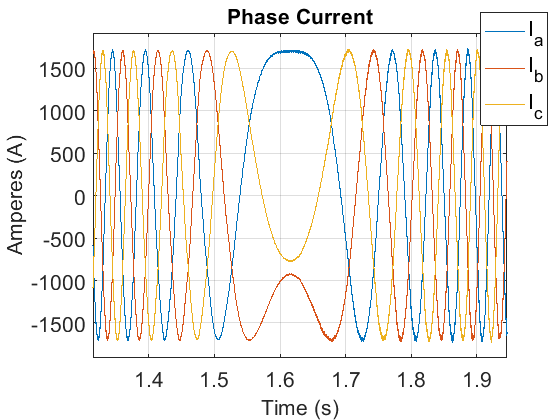
\includegraphics[width = 8 cm]{figs/reverse_phase1.png}
            \caption{Line currents during rotation direction change}
            \label{fig:r22}
        \end{subfigure}
        \caption{Reversal, line currents}
        \label{fig:rev_line1}
        \end{figure}

In the Fig. \ref{fig:dc} below, we can see that our brake resistor starts operating voltage above 560, that is why in steady state we are constrained by 560V. Then, during the reversal due to the current supplied from the motor side, the voltage increases up to 580V, however, braking resistor allows us to discharge this energy. Then, the voltage is decreased to its final value after a transient period. When we have a look at Fig. \ref{fig:sc} we can observe that in steady state both currents are zero with noise, however in the transient time, we have a negative $i_q$ resulted from the motor's reversal. This current discharges over the braking resistance.
        
\begin{figure}[H]
        \centering
        \begin{subfigure}[b]{0.475\textwidth}
            \centering
            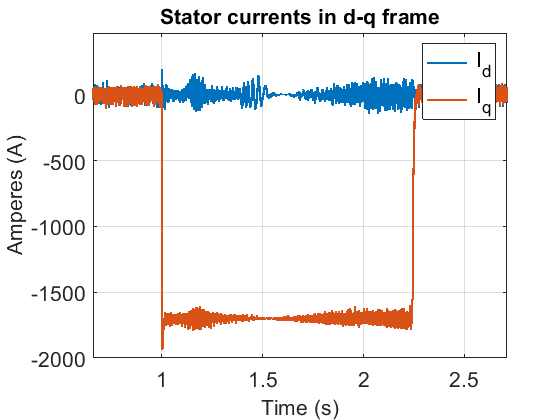
\includegraphics[width = 8 cm]{figs/reverse_dq.png}
            \caption{Stator currents}
            \label{fig:sc}
        \end{subfigure}
        \hfill
        \begin{subfigure}[b]{0.475\textwidth}  
            \centering 
            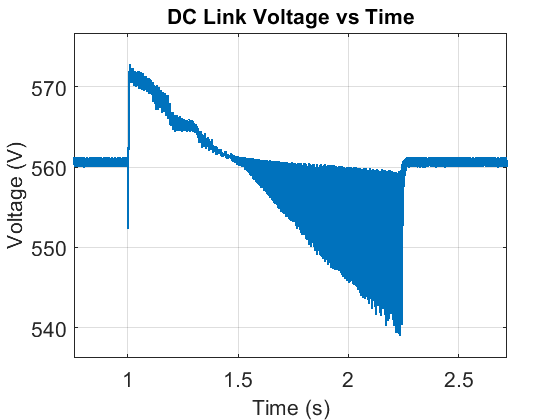
\includegraphics[width = 8 cm]{figs/reverse_dc.png}
            \caption{DC link voltage}
            \label{fig:dc}
        \end{subfigure}
        \caption{Reversal, d-q currents (a) and DC Link voltage (b)}
        \label{fig:dc}
        \end{figure}        




\subsection{Q4}

In this part, we need to operate the motor in the field weakening region. For this calculations, i will apply rated current conditions. In the first state, we are in the rated speed with half of the maximum torque. Since $i_q$ and torque is directly proportional, we can find $i_q$ using these relation. 
\begin{equation}
     i_q = \dfrac{T_{m}}{3 \lambda }
\end{equation}

where Torque can be found as:
$$ T = 1273 Nm$$

When we calculate it:

$$ i_q = \dfrac{1273}{1.5} = 848.7A$$

Since we are in the rated speed, we are in the base region which means there is no need of $i_d$ current to speed up the motor. However when we look at the final operation, i am assuming that we are operating in the rated current conditions over the $i_{s,max}$ line. I do not think that this operation makes sense because there is no need to work on the maximum current line. We will suggest another option below!

$$ i_q = \dfrac{1273}{1.5} = 848.7A$$

$$ i_d = 1700^2 - i_q^2 = 1472A$$

Now, the point is that these values are steady state values, and to speed up the motor we need to apply additional torque in order to speed up, we need a net torque. For this reason, i apply maximum $i_q$ current available at any time, and i add $i_d$ current when the $V$ exceeds its rated value. The results are shown in the following Fig. \ref{fig:b4}


\begin{figure}[H]
        \centering
        \begin{subfigure}[b]{0.475\textwidth}
            \centering
            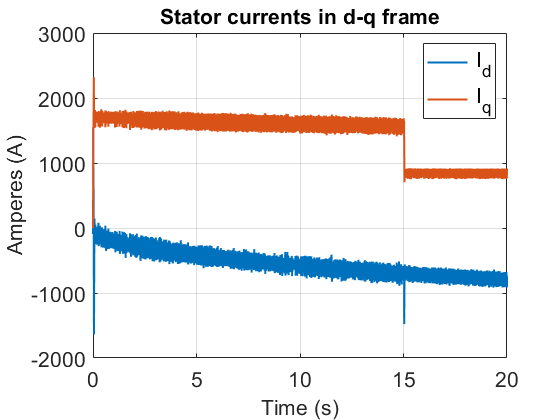
\includegraphics[width = 8 cm]{figs/b4_dq.png}
            \caption{Stator currents}
            \label{fig:b4_dq}
        \end{subfigure}
        \hfill
        \begin{subfigure}[b]{0.475\textwidth}  
            \centering 
            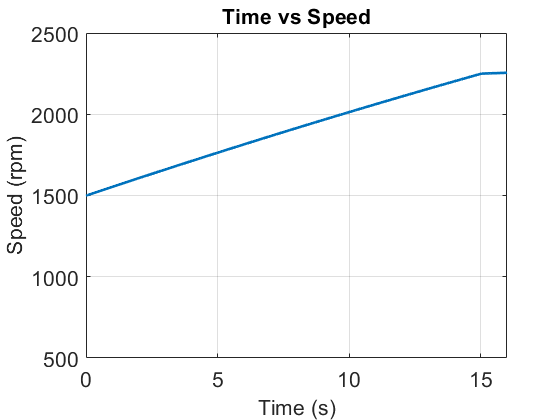
\includegraphics[width = 8 cm]{figs/b4_speed.png}
            \caption{Speed vs time}
            \label{fig:b4_speed}
        \end{subfigure}
        \caption{Field weakening, d-q currents (a) and speed vs time}
        \label{fig:b4}
        \end{figure}    
        
\textbf{Comments:} Normally, in the calculations we made, we found a surprising thing, at the steady state the required $i_d$ current can be calculated in the following limitation:

$$ V_{max} = \sqrt{(\omega_e \lambda + i_d \omega_e L_d)^2 + (i_q \omega_e L_q)^2)}$$

And when we calculate the required minimum current in the steady state we can find the followings: At the 150\% rated speed, the $\omega_e = 471 rad$, 

$$ 270 = \sqrt{235.5 - 0.165i_d)^2 + (140)^2) } $$

So, at this condition we only need $i_d = -28.08A$ if we operate at the rated voltage conditions. However, in the simulations I cannot make it work and I am sharing the numerical results to show that the most logical operation is not the rated current operation, but any other operation with balanced current and voltage. Furthermore, at the transient, we always should supply an $i_d$ current to guarantee that we do not exceed the voltage maximum. It is \textbf{NOT} possible to speed up something applying the amount of torque needed to supply to hold a constant operation. In the simulations, we applied maximum $i_q$ current possible to speed up, and then we hold a constant operation with $i_q$ and $i_d$ at this point.

Below, in the Fig. \ref{fig:b4} we can observe it. As you can see it is possible to apply just $30A$ of $i_d$ current, and hold a steady state operation at 150\% rated speed.

\begin{figure}[H]
        \centering
        \begin{subfigure}[b]{0.475\textwidth}
            \centering
            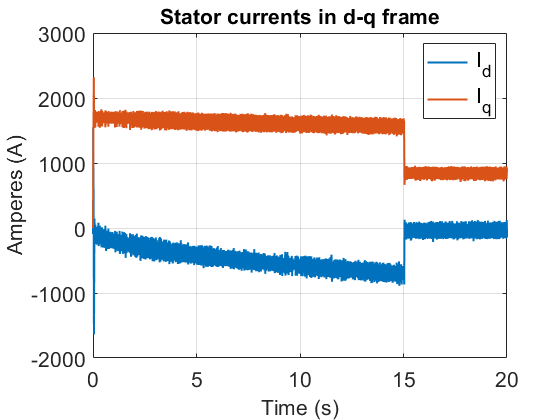
\includegraphics[width = 8 cm]{figs/b4_new_dq.png}
            \caption{Stator currents}
            \label{fig:b4_dq}
        \end{subfigure}
        \hfill
        \begin{subfigure}[b]{0.475\textwidth}  
            \centering 
            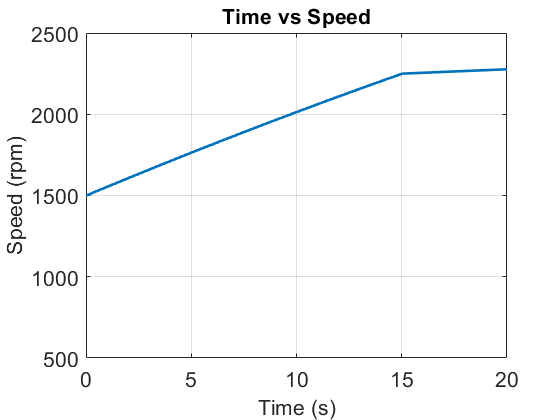
\includegraphics[width = 8 cm]{figs/b4_new_speed.png}
            \caption{Speed vs time}
            \label{fig:b4_speed}
        \end{subfigure}
        \caption{Field weakening, d-q currents (a) and speed vs time}
        \label{fig:b4}
        \end{figure}  
        
This operation is much logical because we do not work in the rated current conditions, it decreases losses and decreases the stress on the equipments. Also, it is not necessary to work on the maximum current line because we are not supplying maximum torque at that speed!